\subsection{Typed cubic completion of the regional ambient space}
\label{vi:cubo:completacion}

The completion admits a set-theoretic description making its operation
explicit. Let \(E_9\) be the set of nine residue classes, represented
positively by \(1,\ldots,9\), and let \(\ast\) be an additional element.
The symbol \(\ast\) differs from the zero class, already represented by \(9\).
Consequently, extending \(E_9\) to
\(\widehat E=E_9\sqcup\{\ast\}\) increases the cardinality from nine
to ten without changing the internal modular identification. The cubic
completion is \(\widehat C=\widehat E^3\), and the initial cube is \(C=E_9^3\).

The regional ambient space already constructed by \(\Psi\) in
\eqref{eq:psi-catalogo}, whose exact census is established in
Proposition~\ref{vi:reg:censo}, is \(\FF_3^6\). To type its residence in
the initial cube, write
\([a]_3\in\{0,1,2\}\) for the representative of \(a\in\FF_3\) and fix
the bijection
\[
 \eta:\FF_3^2\longrightarrow E_9,
 \qquad \eta(a,b)=1+3[a]_3+[b]_3.
\]
Pairwise grouping gives
\begin{equation}
 \beta(w_1,\ldots,w_6)=
 \bigl(\eta(w_1,w_2),\eta(w_3,w_4),\eta(w_5,w_6)\bigr)
 \label{vi:cubo:beta}
\end{equation}
and is therefore a bijection \(\FF_3^6\to E_9^3=S_0\). In particular,
the \(243\) words produced by the preceding census reside in the initial
body of \(729\) positions; neither \(\eta\) nor \(\beta\) selects a
region, a physical species, or a metrological value. Regional selection
is a later and distinct stage, proved in
Proposition~\ref{vi:reg:seleccion}. The numerical equality
\(|\operatorname{im}\Psi|=|S_1|=243\) does not identify the two sets:
\(\beta(\operatorname{im}\Psi)\) is a subset of \(S_0\), whereas
\(S_1\) belongs to the expansion shell.

\subsubsection{Threshold difference and composition of shells}
\label{vi:cube:mg07:threshold}

The enlargement of a discrete cell preserves every stratum appearing
when its size increases by one unit. The threshold difference expresses
this operation on the cardinality reader and tracks its behaviour under
addition and multiplication before a metric realization is introduced.

\begin{definition}[Threshold difference]
Let \(R\) be a commutative ring with identity and let
\(f:\mathbb Z_{\geq0}\to R\). Define
\begin{equation}
 (D_\#f)(n)=f(n+1)-f(n).
 \label{vi:cube:mg07:definition}
\end{equation}
For an integer reader of nested finite cells, this difference records
the cardinality of the shell added in the step \(n\to n+1\).
\end{definition}

\begin{proposition}[Additivity and exact product law]
For \(f,g:\mathbb Z_{\geq0}\to R\),
\begin{align}
 D_\#(f+g)(n)&=D_\#f(n)+D_\#g(n),
 \label{vi:cube:mg07:additivity}\\
 D_\#(fg)(n)&=f(n+1)D_\#g(n)+g(n)D_\#f(n)
 \label{vi:cube:mg07:shifted-product}\\
 &=f(n)D_\#g(n)+g(n)D_\#f(n)
   +D_\#f(n)D_\#g(n).
 \label{vi:cube:mg07:product}
\end{align}
\end{proposition}

\begin{proof}
The difference of a sum separates term by term. For the product,
adding and subtracting \(f(n+1)g(n)\) gives
\[
 \begin{split}
 f(n+1)g(n+1)-f(n)g(n)
 &=f(n+1)\bigl(g(n+1)-g(n)\bigr)\\
 &\quad+g(n)\bigl(f(n+1)-f(n)\bigr).
 \end{split}
\]
This proves \eqref{vi:cube:mg07:shifted-product}. Substitution of
\(f(n+1)=f(n)+D_\#f(n)\) yields \eqref{vi:cube:mg07:product}, including
its complete bilinear term.
\end{proof}

If \(A_n\subseteq A_{n+1}\) and \(B_n\subseteq B_{n+1}\) are
finite sets, the shell of the product decomposes into three disjoint
parts:
\[
 \begin{split}
 (A_{n+1}\times B_{n+1})\setminus(A_n\times B_n)
 &=\bigl(A_n\times(B_{n+1}\setminus B_n)\bigr)\\
 &\quad\sqcup\bigl((A_{n+1}\setminus A_n)\times B_n\bigr)\\
 &\quad\sqcup\bigl((A_{n+1}\setminus A_n)
                 \times(B_{n+1}\setminus B_n)\bigr).
 \end{split}
\]
Taking cardinalities gives exactly \eqref{vi:cube:mg07:product}. The
bilinear term counts positions new in both factors; it resides in
the intersection of the two enlargements, with incidence preserved.

\begin{proposition}[Binomial law for the dimensional shell]
For \(d\geq1\), let \(f_d(n)=n^d\). Then
\begin{equation}
 D_\#f_d(n)=(n+1)^d-n^d
 =\sum_{k=0}^{d-1}\binom dk n^k
 =\sum_{r=1}^{d}\binom dr n^{d-r}.
 \label{vi:cube:mg07:binomial}
\end{equation}
\end{proposition}

\begin{proof}
The binomial expansion of \((n+1)^d\) contains \(n^d\) and the
remaining \(d\) terms in the first sum. Substituting \(r=d-k\)
gives the second sum. In the support \(\{1,\ldots,n+1\}^d\),
each added position has a nonempty set of coordinates equal to
\(n+1\). If that set has \(r\) elements, there are \(\binom dr\)
choices of positions and \(n^{d-r}\) choices of previous coordinate
values. These strata are disjoint and cover the shell, also proving
the formula by finite incidence.
\end{proof}

For \(d=3\), the three strata have cardinalities \(3n^2\),
\(3n\), and \(1\). At the nonadic--decimal step, \(n=9\), the
operation gives \(243+27+1=271\); excluding the final vertex leaves
\(270\) positions. The following cubic completion makes explicit
the union of this shell with the \(729\) previous positions. The
threshold law thus preserves both the total and its distribution by
the number of new coordinates. Subsequent lattice realizations
transport their incidences through the maps specific to each
construction.


\begin{definition}[Strata of combinatorial codimension]
For \(0\leq r\leq3\), define
\[
 S_r=\{(x_1,x_2,x_3)\in\widehat E^3:
             \#\{j:x_j=\ast\}=r\}.
\]
The apex of the completion is \(a_\ast=(\ast,\ast,\ast)\), and the
punctured completion is \(\widehat C^{\circ}=\widehat C\setminus\{a_\ast\}\).
\end{definition}

\begin{proposition}[Exact decomposition of the completion]
The strata are disjoint and satisfy
\begin{align}
 \widehat C&=S_0\sqcup S_1\sqcup S_2\sqcup S_3,
 &|S_r|&=\binom3r9^{3-r},\label{vi:cubo:estratos}\\
 |\widehat C^{\circ}|&=729+243+27=999,
 &|\widehat C|&=999+1=729+271=1000.\label{vi:cubo:999}
\end{align}
The punctured expansion contains \(270\) elements in addition to the
initial cube; the complete expansion contains \(271\).
\end{proposition}
\begin{proof}
An element of \(S_r\) is obtained by choosing the \(r\) coordinates
containing \(\ast\), in \(\binom3r\) ways, and assigning one of the
nine classes of \(E_9\) to each remaining coordinate. Classification by
the number of additional coordinates is exhaustive and its classes are
disjoint. The sole element of \(S_3\) is \(a_\ast\). Removing it
subtracts one from the total cardinality; restoring it recovers the
complete Cartesian product.
\end{proof}

The expression \emph{holographic extreme and mean ratio}, abbreviated EMRH
in the corpus, here denotes this articulation of the initial body, expansion
strata, and unit restoration. Its immediate content is the exact partition
of a finite product and its normalization. The number \(999\) represents
a definite object, the punctured completion; \(1000\) represents its
closure through restoration of the apex. The added unit therefore has
an explicit incidence location.

\begin{figure}[htbp]
\centering
\begin{tikzpicture}[x=1cm,y=1cm,>=Stealth,font=\small]
\draw[->] (0,0)--(12.4,0);
\foreach \x/\a/\b in {0/729/{S_0},4.0/243/{S_1},7.5/27/{S_2},10.6/1/{S_3}}{
  \draw (\x,0.12)--(\x,-0.12);
  \node[above=5pt] at (\x,0) {\(\a\)};
  \node[below=5pt] at (\x,0) {\(\b\)};
}
\draw[decorate,decoration={brace,amplitude=5pt}] (0,1)--(7.7,1);
\node[above=8pt] at (3.85,1) {Punctured completion: \(999\)};
\draw[decorate,decoration={brace,mirror,amplitude=5pt}] (0,-1)--(10.8,-1);
\node[below=8pt] at (5.4,-1) {Full completion: \(1000=999+1\)};
\node[align=center] at (10.6,1.5) {Apex\\\((\ast,\ast,\ast)\)};
\end{tikzpicture}
\caption{Strata of the cubic completion. The arrangement represents
the set-theoretic decomposition, not a metric scale. The \(243\) elements
of \(S_1\) form three coordinate strata of \(81\) elements; the \(27\)
elements of \(S_2\) form three strata of \(9\). The apex completes the partition.}
\label{vi:cubo:estratos-fig}
\end{figure}

% Inclusion of the historical vector figure in greyscale.
% The PDF and its standalone source are preserved verbatim as cubo_emrh_original.*.
\begin{figure}[htbp]
\centering
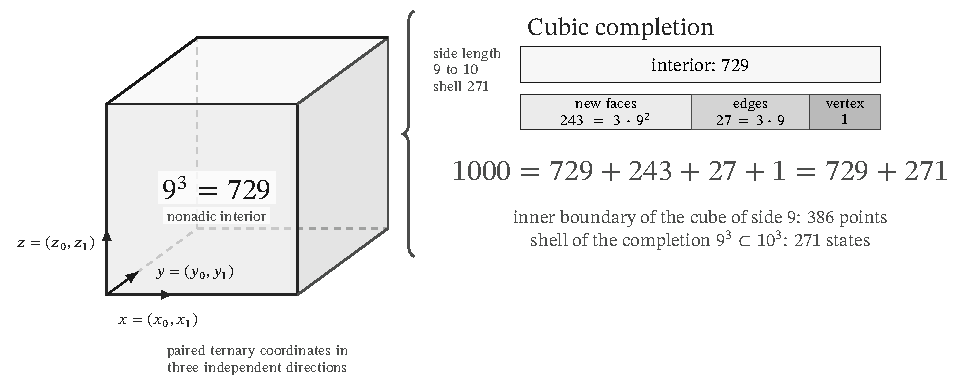
\includegraphics[width=\textwidth]{figures/cubo_emrh_original.pdf}
\caption{Cubic representation of the expansion from nine to ten classes per coordinate. Strata \(S_1,S_2,S_3\) locate the added incidences on faces, edges, and the apex; their cardinalities form the \(271\)-element shell. The \(386\)-element boundary belongs to the initial cube. This geometric perspective complements the partition in Figure~\ref{vi:cubo:estratos-fig}; graphical spacing is schematic.}
\label{vi:cubo:completacion-3d}
\end{figure}


\subsubsection{Conservation of unity and dimensional compatibility}

Normalization is not limited to dividing an isolated identity. In dimension
\(d\), the product \(\widehat E^d\) carries the uniform measure
\(\mu_d(\{x\})=10^{-d}\). The coordinate projection
\(p_d:\widehat E^{d+1}\to\widehat E^d\) deletes the last coordinate.

\begin{proposition}[Projective compatibility of normalized measures]
For every \(d\geq1\),
\[
 (p_d)_*\mu_{d+1}=\mu_d,
 \qquad \mu_d(\widehat E^d)=1.
\]
The mass of the stratum with \(r\) additional coordinates is
\(\binom dr9^{d-r}/10^d\), and the masses of all strata sum to one.
\end{proposition}
\begin{proof}
Each point of \(\widehat E^d\) has ten preimages. Their total mass is
\(10\,10^{-(d+1)}=10^{-d}\). Equality for any subset follows by
summing over its points. The stratified formula follows from the same
count as \eqref{vi:cubo:estratos}; the binomial
\((9+1)^d\) gives total normalization.
\end{proof}

In dimension three, removing the apex leaves mass \(999/1000\), and
restoring it adds \(1/1000\). Renormalizing before restoration would
define a different measure: the distinction is operationally relevant.
In particular, conservation of probability mass, conservation of transport
records, and thermodynamic dissipation concern different objects. The
proposition proves the first and provides the compatible support for
studying the second; the third requires a specified dynamic and energetic realization.

The internal geometric boundary also remains distinct.
On the Cartesian representative \(\{1,\ldots,9\}^3\), removing
\(\{2,\ldots,8\}^3\) leaves \(386\) points. This boundary belongs
to the initial cube, whereas \(\widehat C\setminus C\) belongs to
its expansion. Cubic completion, base-thousand positional expansion,
and exceptional-incidence reading share support data; their respective
maps determine which information from these data each representation uses.
